%; whizzy section -pdf xpdf -latex ./whizzypdfptex.sh
% latex beamer presentation.
% platex, latex-beamer $B$G%3%s%Q%$%k$9$k$3$H$rA[Dj!#(B 

%     Tokyo Debian Meeting resources
%     Copyright (C) 2008 Junichi Uekawa

%     This program is free software; you can redistribute it and/or modify
%     it under the terms of the GNU General Public License as published by
%     the Free Software Foundation; either version 2 of the License, or
%     (at your option) any later version.

%     This program is distributed in the hope that it will be useful,
%     but WITHOUT ANY WARRANTY; without even the implied warranty of
%     MERCHANTABILITY or FITNESS FOR A PARTICULAR PURPOSE.  See the
%     GNU General Public License for more details.

%     You should have received a copy of the GNU General Public License
%     along with this program; if not, write to the Free Software
%     Foundation, Inc., 51 Franklin St, Fifth Floor, Boston, MA  02110-1301 USA

\documentclass[cjk,dvipdfm,12pt]{beamer}
\usetheme{Tokyo}
\usepackage{ulem}
\usepackage{tabularx}

\usepackage{fancybox}
\usepackage{fancyvrb}   
\usepackage{float}

% commandline$B4D6-$rDj5A!#2hLLF~=PNO$K$D$$$F$O(Bcommandline$B4D6-(B
% $B$GI=5-$9$k(B
\newenvironment{commandline}%
{\VerbatimEnvironment
  \begin{Sbox}\begin{minipage}{0.9\hsize}\begin{fontsize}{7.3}{7.3} \begin{BVerbatim}}%
{\end{BVerbatim}\end{fontsize}\end{minipage}\end{Sbox}
  \setlength{\fboxsep}{8pt}
% start on a new paragraph

\vspace{6pt}% skip before
\fcolorbox{dancerdarkblue}{dancerlightblue}{\TheSbox}

\vspace{6pt}% skip after
}
%end of commandline

\definecolor{dancerdarkblue}{rgb}{0,0.08,0.45}
\definecolor{dancernormalblue}{rgb}{0.8,0.9,0.95}
\definecolor{dancerlightblue}{rgb}{0.8,0.95,1}


%  preview (shell-command (concat "evince " (replace-regexp-in-string "tex$" "pdf"(buffer-file-name)) "&"))
%  presentation (shell-command (concat "xpdf -fullscreen " (replace-regexp-in-string "tex$" "pdf"(buffer-file-name)) "&"))

%http://www.naney.org/diki/dk/hyperref.html
%$BF|K\8l(BEUC$B7O4D6-$N;~(B
\AtBeginDvi{\special{pdf:tounicode EUC-UCS2}}
%$B%7%U%H(BJIS$B7O4D6-$N;~(B
%\AtBeginDvi{\special{pdf:tounicode 90ms-RKSJ-UCS2}}

\title{$BEl5~%(%j%"(B Debian $BJY6/2q(B}
\subtitle{$B;qNA(B}
\author{$B>e@n(B $B=c0l(B dancer@debian.org\\IRC nick: dancerj}
\date{2008$BG/(B3$B7n(B15$BF|(B}
\logo{
\includegraphics[width=8cm]{image200607/openlogo-light.eps}}


% $B4V$N%?%$%H%k%Z!<%8MQ(B
\newcommand{\emtext}[1]{
\begin{frame}{}
 
\begin{minipage}{0.55\hsize}
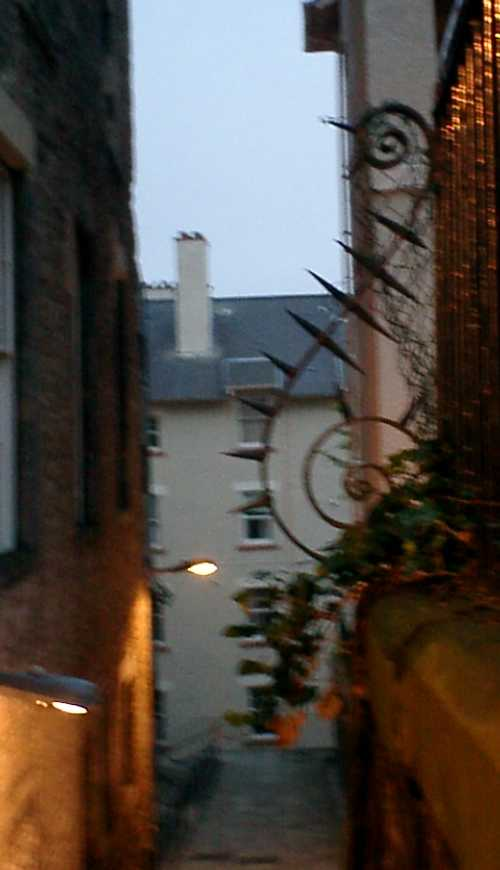
\includegraphics[width=1\hsize]{image200707/gurutitle.jpg}
\end{minipage}
\begin{minipage}{0.39\hsize}
 {\Huge #1
 }
\end{minipage}
\end{frame}
}

% $B;0BrLdBjMQ(B
\newcounter{santakucounter}
\newcommand{\santaku}[5]{%
\addtocounter{santakucounter}{1}
\frame{\frametitle{$BLdBj(B\arabic{santakucounter}. #1}
%$BLdBj(B\arabic{santakucounter}. #1
\begin{minipage}[t]{0.8\hsize}
 \begin{itemize}
 \item
      \begin{minipage}{0.2\hsize}
      
\includegraphics[width=0.9\hsize]{image200703/janken-A.png}\end{minipage} 
       \begin{minipage}{0.6\hsize}
       A #2\end{minipage}\\
 \item
      \begin{minipage}{0.2\hsize}
      
\includegraphics[width=0.9\hsize]{image200703/janken-B.png}\end{minipage} 
       \begin{minipage}{0.6\hsize}
       B #3\end{minipage}\\
 \item
      \begin{minipage}{0.2\hsize}
      
\includegraphics[width=0.9\hsize]{image200703/janken-C.png}\end{minipage} 
       \begin{minipage}{0.6\hsize}
       C #4\end{minipage}\\
 \end{itemize}
\end{minipage}
}
\frame{\frametitle{$BLdBj(B\arabic{santakucounter}. #1}
%$BLdBj(B\arabic{santakucounter}. #1
\begin{minipage}[t]{0.8\hsize}
\begin{itemize}
 \item
      \begin{minipage}{0.2\hsize}
      
\includegraphics[width=0.9\hsize]{image200703/janken-A.png}\end{minipage} 
       \begin{minipage}{0.6\hsize}
       A #2\end{minipage}\\
 \item
      \begin{minipage}{0.2\hsize}
      
\includegraphics[width=0.9\hsize]{image200703/janken-B.png}\end{minipage} 
       \begin{minipage}{0.6\hsize}
       B #3\end{minipage}\\
 \item
      \begin{minipage}{0.2\hsize}
      
\includegraphics[width=0.9\hsize]{image200703/janken-C.png}\end{minipage} 
       \begin{minipage}{0.6\hsize}
       C #4\end{minipage}\\
\end{itemize}
\end{minipage}
\begin{minipage}[t]{0.15\hsize}
$BEz$($O(B:

\vspace{1cm}

  {\huge \hspace{1cm}#5}
  \hspace{-6cm}\includegraphics[width=4cm]{image200703/janken-#5.png}
 \end{minipage}}
}

\begin{document}

\frame{\titlepage{}}


\section{Intro}

\emtext{$B@_1D=`Hw$K$46(NO$/$@$5$$(B}

\begin{frame}
 \frametitle{Agenda}
\begin{minipage}[t]{0.45\hsize}
  \begin{itemize}
  \item $BCm0U;v9`(B
	\begin{itemize}
	 \item $B;#1F6X;_(B
	 \item $B$3$NIt20$GOC$5$l$?$3$H$O$3$NIt20$N30$K$O0lJb$b=P$^$;$s(B
	\end{itemize}
  \item quiz
  \item $B:G6a$N(BDebian$B4XO"$N%$%Y%s%H(B
	\begin{itemize}
	 \item $BA0!92s(B
	 \item $BA02s(B $B!J(BOSC$B!K(B
	\end{itemize}
 \end{itemize}
\end{minipage} 
\begin{minipage}[t]{0.45\hsize}
 \begin{itemize}
  \item $B%G!<%?$@$1$N(BDebian$B%Q%C%1!<%8(B
  \item Debian$B$G$N%i%$%;%s%9$N9M$(J}(B
 \end{itemize}
\end{minipage}
\end{frame}

\section{$B:G6a(B}

\begin{frame}
 \frametitle{$BA0!92s$N(BAgenda}
\begin{minipage}[t]{0.45\hsize}
  \begin{itemize}
  \item $BCm0U;v9`(B
	\begin{itemize}
	 \item $B0{?)6X;_(B
	 \item $B@/<#(B/$B=!65(B/$B1DMx3hF06X;_(B
	\end{itemize}
  \item quiz
  \item $B:G6a$N(BDebian$B4XO"$N%$%Y%s%H(B
	\begin{itemize}
	 \item $BA02s(B
	\end{itemize}
 \end{itemize}
\end{minipage} 
\begin{minipage}[t]{0.45\hsize}
 \begin{itemize}
  \item 2008$BG/EY(B Debian $BJY6/2q4k2h(B
  \item Debian Package $B4IM}$NN.$l(B
 \end{itemize}
\end{minipage}
\end{frame}


\begin{frame}{Git $BFC=8(B}

Debian$BJY6/2q$N%j%]%8%H%j$O(BGit$B4IM}$G$9!#(B
Git$B$N;H$$J}$,$o$+$i$J$$$H$$$C$F$$$kJ}!9!"$h$s$G$*$$$F$/$@$5$$!#(B


\includegraphics[width=0.5\hsize]{image200803/gihyo200804.jpg}

\end{frame}


\section{Debian$BJY6/2q$H$O(B}
\emtext{Debian$BJY6/2q$H$O(B}
\begin{frame}{Debian$BJY6/2q$H$O(B}
$B8l$C$F$_$k!#(B
\end{frame}


\section{DWN quiz}
\begin{frame}{Debian $B>o<1%/%$%:(B}

Debian $B$N>o<1!"$b$A$m$sCN$C$F$^$9$h$M(B?
$BCN$i$J$$$J$s$FCQ$:$+$7$/$F!"CN$i$J$$$H$O8@$($J$$$"$s$J$3$H$d$3$s$J$3$H!"(B
$B$_$s$J$G3NG'$7$F$_$^$7$g$&!#(B

$B:#2s$N=PBjHO0O$O!"(B\url{http://lists.debian.org/debian-devel-announce/} $B$K$"$k:G6a$N(B
$B%"%J%&%s%9J8=q$G$9!#(B

\end{frame}

\subsection{$BLdBj(B}

%$BLdBj$r%3%T%Z(B

\section{$B:G6a$NOCBj(B}

\emtext{OSC$B;22CJs9p(B}

\section{$B;vA02]Bj>R2p(B}
\emtext{$B;vA02]Bj$N>R2p(B}
% pre work home work

\begin{frame}{$B;vA02]BjLdBj(B}

\begin{enumerate}
 \item $B%G!<%?$@$1$N%Q%C%1!<%8$G$G$-$k$3$H(B
 \item $B%=%U%H%&%'%"$N%i%$%;%s%9$GIT<+M3$7$?$3$H(B
 \item $B9%$-$J%=%U%H%&%'%"%i%$%;%s%9$H$=$NM}M3(B
\end{enumerate}

\end{frame}

% (query-replace "\\subsection" "\\end{frame}\\begin{frame}")
% (query-replace "\\subsubsection" "\\textbf")

\emtext{2008$BG/7W2h(B}

\begin{frame}{2008$BG/7W2h(B}

{\scriptsize
\begin{enumerate}
 \item $B?7G/2q!V5$9g$rF~$l$k!W(B
 \item Open Source Conference Tokyo (3/1)
 \item $B%G!<%?$@$1$N%Q%C%1!<%8$r:n@.$7$F$_$k!"(B
       $B%i%$%;%s%9$N9M$(J}(B (David Smith)
 \item $B%P%$%J%j0l$D$N%Q%C%1!<%8$r:n@.$7$F$_$k(B ($B5HED(B@$BHD66(B)\\
       $B%P!<%8%g%s4IM}%D!<%k$r;H$$(BDebian$B%Q%C%1!<%8$r4IM}$9$k(B(git)\\
       $B%"%C%W%9%H%j!<%`$N07$$(B(svn/git/cvs)($B4d>>(B $B?.MN$5$s(B)
 \item $B%P%$%J%j$NJ,$1$?%Q%C%1!<%8$N:n@.!#(B($BA0ED$5$s(B)\\
       $B%P%$%J%j$NJ,$1J}$N9M$(J}!"%"%C%W%0%l!<%I$J$I$N1?MQ$H$+!#(B
 \item $B%Q%C%1!<%8:n@.(B(dpatch/debhelper$B$G:n@.$9$k%Q%C%1!<%8(B)($B>.NS576)$5$s(B)\\
       man $B$N=q$-J}(B(roff or docbook)($B$G$s$5$s(B)
 \item $B%Q%C%1!<%8:n@.(B(kernel patch$B!"(Bkernel module)
       $B!"(BDebconf$BH/I=N}=,(B
 \item Debconf $B%"%k%<%s%A%s!"6&M-%i%$%V%i%j%Q%C%1!<%8:n@.(B

 \item Open Source Conference Tokyo/Fall$B!"(B
       $B%G!<%b%s7O$N%Q%C%1!<%8$N:n@.!"(Blatex$B!"(B emacs-lisp$B!"%U%)%s%H%Q%C%1!<%8(B
 \item $B%Q%C%1!<%8$N(B cross-compile $B$NJ}K!!"(Bamd64 $B>e$G(B i386 $B$N%Q%C%1!<%8$H(B
       $B$+!"(BOSC-Fall$BJs9p2q!"(BDebconf$BJs9p2q(B
 \item $B9q:]2=(B po-debconf / po$B2=(B / DDTP
 \item $BK:G/2q(B
\end{enumerate}
}
\end{frame}

\emtext{$B%G!<%?$@$1$N%Q%C%1!<%8:n@.(B}

\emtext{Debian$B$G$N%=%U%H%&%'%"%i%$%;%s%9$N9M$(J}(B}
\section{Debian$B$G$N%=%U%H%&%'%"%i%$%;%s%9$N9M$(J}(B}


\begin{frame}{$B%i%$%;%s%9$NJ,N`(B?}

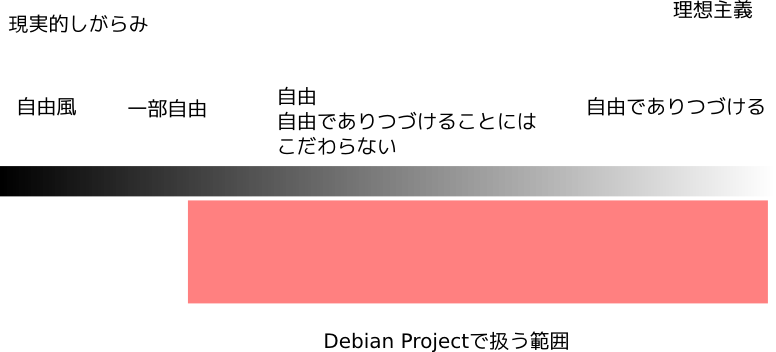
\includegraphics[width=1.1\hsize]{image200803/freerange.png}
\end{frame}

\begin{frame}{$BBg;(GD$K<+M3$J%i%$%;%s%9$NN`7?$G$o$1$F$_$k(B}
\begin{itemize}
 \item $B<+M3$J$b$N$r<+M3$G$"$j$D$E$1$5$;$?$$%i%$%;%s%9!J(BGPL$B$J$I!K(B
 \item $B<+M3$J$b$N$rIT<+M3$K$9$k<+M3$bM?$($?$$%i%$%;%s%9!J(BMIT, BSD$B$J$I!K(B
 \item $B<+J,$N:n$C$?$b$N$O<+M3$K$D$+$C$F$/$l$F$h$$$,!"<+J,$N:n@.$7$?$b$N(B
       $B$O40A4$J$?$a!">!<j$K$$$8$C$F$[$7$/$J$$!#$h$C$F!"JQ99$7$?$b$N$K$D$$$F(B
       $B$OL@<(E*$K$7$F$*$$$F$[$7$$$b$N!J(BLPPL 1.0$B$J$I!K(B
\end{itemize}
\end{frame}
\begin{frame}{Debian Project$B$G$N;H$o$lJ}(B}
\begin{itemize}
 \item Debian $B$rM-=~!&L5=~$rLd$o$:G[I[$9$k$3$H!J(BDVD$B!&8x3+%_%i!<!&Hs8x3+(B
       $B%_%i!<!K(B
 \item Debian $B$r2~JQ$9$k$3$H!J(BDebian$B$N2~NI!"(BDebian$B30$X$NN.MQ!"(BDebian$B$+$i(B
       $B$NGI@8%G%#%9%H%j%S%e!<%7%g%s$N3+H/$J$I!K(B
 \item Debian$B$r$"$i$f$kMQES$GMxMQ$G$-$k$3$H!J>&MQ!&650iMQ!&=!65MQ!&73;v(B
       $BMQ!&0eNEMQ$J$I$rLd$o$J$$!K(B
\end{itemize}
\end{frame}

\begin{frame}{DFSG 1/2}

 {\scriptsize

     1. Free Redistribution

       The license of a Debian component may not restrict any party from
       selling or giving away the software as a component of an aggregate
       software distribution containing programs from several different
       sources. The license may not require a royalty or other fee for
       such sale.

    2. Source Code

       The program must include source code, and must allow distribution
       in source code as well as compiled form.

    3. Derived Works

       The license must allow modifications and derived works, and must
       allow them to be distributed under the same terms as the license
       of the original software.

    4. Integrity of The Author's Source Code

       The license may restrict source-code from being distributed in
       modified form {\bf only} if the license allows the distribution of
       "patch files" with the source code for the purpose of modifying
       the program at build time. The license must explicitly permit
       distribution of software built from modified source code. The
       license may require derived works to carry a different name or
       version number from the original software. (This is a compromise.
       The Debian group encourages all authors not to restrict any files,
       source or binary, from being modified.)

    5. No Discrimination Against Persons or Groups

       The license must not discriminate against any person or group of
       persons.

}
\end{frame}
\begin{frame}{DFSG 2/2}

{\scriptsize
    6. No Discrimination Against Fields of Endeavor

       The license must not restrict anyone from making use of the
       program in a specific field of endeavor. For example, it may not
       restrict the program from being used in a business, or from being
       used for genetic research.

    7. Distribution of License

       The rights attached to the program must apply to all to whom the
       program is redistributed without the need for execution of an
       additional license by those parties.

    8. License Must Not Be Specific to Debian

       The rights attached to the program must not depend on the
       program's being part of a Debian system. If the program is
       extracted from Debian and used or distributed without Debian but
       otherwise within the terms of the program's license, all parties
       to whom the program is redistributed should have the same rights
       as those that are granted in conjunction with the Debian system.

    9. License Must Not Contaminate Other Software

       The license must not place restrictions on other software that is
       distributed along with the licensed software. For example, the
       license must not insist that all other programs distributed on the
       same medium must be free software.

   10. Example Licenses

       The "GPL", "BSD", and "Artistic" licenses are examples of licenses
       that we consider "free".
 }
\end{frame}

\begin{frame}{Debian $B%Q%C%1!<%8$N%i%$%;%s%94IM}(B}

$BH/@8$9$k%$%Y%s%H(B
\begin{itemize}
 \item ITP
 \item New queue
 \item $B:FG[I[(B
 \item $B2~JQ(B
\end{itemize}
\end{frame}

\begin{frame}{debian/copyright}
\begin{itemize}
 \item README
 \item SOURCE
 \item BINARY
\end{itemize} 
\end{frame}



\section{}

\begin{frame}{$B1c2q>l=j(B}

\begin{itemize}
 \item $B1c2q>l=j(B\\
       $BK\F|$N1c2q$O!V0C(BGuRi$B!J$"$0$j!K(B 5566$B!W$G$9!#(B
       $BD>A0$K?M?t$r3NDj$7$F(B 03-3780-5566 $B$KEEOC$7$F$/$@$5$$$H0MMj$5$l$F$$$k$N$GEEOC$7$^$9!#(B\\
       $B;22C<T$O(BB1F$B$K=89g$7!"A40w$G0\F0$7$^$7$g$&!#(B
 \item $BJRIU$1(B\\
       $BIt20$rJRIU$1$k$N$K$46(NO$/$@$5$$!#(B
\end{itemize}

\end{frame}

\end{document}

;;; Local Variables: ***
;;; outline-regexp: "\\([ 	]*\\\\\\(documentstyle\\|documentclass\\|emtext\\|section\\|begin{frame}\\)\\*?[ 	]*[[{]\\|[]+\\)" ***
;;; End: ***
